\documentclass[a4paper,10pt]{article}

%Math
\usepackage{amsmath}
\usepackage{amsfonts}
\usepackage{amssymb}
\usepackage{amsthm}
\usepackage{ulem}
\usepackage{stmaryrd} %f\UTF{00FC}r Blitz!

%PageStyle
\usepackage[german]{babel}
\usepackage{fontenc}
\usepackage{fancyhdr, graphicx}
\usepackage{wasysym}
\usepackage{fullpage}
\usepackage{textcomp}
\usepackage{fancyhdr} %for header/footer

%My Commands
\newcommand{\BN}{\mathbb{B}} %BOOL
\newcommand{\RN}{\mathbb{R}} %Real Number
\newcommand{\NN}{\mathbb{N}} %Natural Number
\newcommand{\QN}{\mathbb{Q}} %Rational Number
\newcommand{\ZN}{\mathbb{Z}} %ganze Zahlen
\newcommand{\CN}{\mathbb{C}}
\newcommand{\Teilt}{\mid} %|
\newcommand{\Teiltn}{\nmid} %kein teiler
\newcommand{\Potp}{\mathcal{P}} %Potenzmenge
\newcommand{\Pota}{\mathcal{A}}
\newcommand{\Potr}{\mathcal{R}}
\newcommand{\Potn}{\mathcal{N}}
\newcommand{\Bold}[1]{\textbf{#1}} %Boldface
\newcommand{\Kursiv}[1]{\textit{#1}} %Italic
\newcommand{\T}[1]{\text{#1}} %Textmode
\newcommand{\Nicht}[1]{\T{\sout{$ #1 $}}} %Streicht Shit durch
\newcommand{\lra}{\leftrightarrow} %Arrows
\newcommand{\ra}{\rightarrow}
\newcommand{\la}{\leftarrow}
\newcommand{\lral}{\longleftrightarrow}
\newcommand{\ral}{\longrightarrow}
\newcommand{\lal}{\longleftarrow}
\newcommand{\Lra}{\Leftrightarrow}
\newcommand{\Ra}{\Rightarrow}
\newcommand{\La}{\Leftarrow}
\newcommand{\Lral}{\Longleftrightarrow}
\newcommand{\Ral}{\Longrightarrow}
\newcommand{\Lal}{\Longleftarrow}
\newcommand{\Vektor}[1]{\vec{#1}}
\newcommand{\Brace}[1]{\left( #1 \right)} %()
\newcommand{\Bracel}[1]{\left\lbrace #1 \right.} %(
\newcommand{\Bracer}[1]{\right. #1 \right\rbrace} %)
\newcommand{\Brack}[1]{\left\lbrace #1 \right\rbrace} %{}
\newcommand{\Brackl}[1]{\left\lbrace #1 \right.} %{
\newcommand{\Brackr}[1]{\right. #1 \right\rbrace} %}
\newcommand{\Result}[1]{\underline{\underline{#1}}} %Doppelt unterstrichen
\newcommand{\Abs}[1]{\left| #1 \right|} %Absolutbetrag
\newcommand{\Norm}[1]{\Abs{\Abs{ #1 }}} %Norm
\newcommand{\Arrays}[1]{\left(\begin{array}{c}#1\end{array}\right)} %Array mit einer Kolonne ()
\newcommand{\Array}[2]{\left(\begin{array}{#1}#2\end{array}\right)} %Array mit n Kolonnen ()
\newcommand{\Bracka}[2]{\left\lbrace\begin{array}{#1}#2\end{array}\right\rbrace} %Array mit {}
\newcommand{\Brackal}[2]{\left\lbrace\begin{array}{#1} #2 \end{array}\right.} %Array mit {
\newcommand{\Brackar}[2]{\left.\begin{array}{#1} #2 \end{array}\right\rbrace} %Array mit }
\newcommand{\Sumone}[2]{\sum_{#2=1}^{#1}} %Summe von 1
\newcommand{\Sumz}[2]{\sum_{#2=0}^{#1}} %Summe von 0
\newcommand{\Sum}[2]{\sum_{#2}^{#1}} %Allgemeine Summe
\newcommand{\Oneover}[1]{\frac{1}{#1}} %1 \UTF{00FC}ber igendwas
\newcommand{\Tablewt}[3]{\begin{table*}[h]\caption{#1} \begin{tabular}{#2}{#3}\end{tabular}\end{table*}} %Table mit Titel
\newcommand{\Oben}[2]{\overset{#1}{#2}} %etwas \UTF{00FC}ber etwas anderem
\newcommand{\Unten}[2]{\underset{#1}{#2}} %etwas unter etwas anderem
\newcommand{\Bildcap}[2]{\begin{figure}[htb]\centering\includegraphics[width=0.2\textwidth]{#1} \caption{#2}\end{figure}} %Bild mit beschriftung
\newcommand{\Bildjpeg}[1]{\includegraphics[width=0.2\textwidth]{#1.jpeg}} %Bilder jpeg!!
\newcommand{\Bildjpg}[1]{\includegraphics[width=0.2\textwidth]{#1.jpg}} %Bilder jpg!!

%Zeichnung
\usepackage{tikz}
\usepackage[all]{xy}
\usepackage{ucs}

\definecolor{dkgreen}{rgb}{0,0.6,0}
\definecolor{gray}{rgb}{0.5,0.5,0.5}
\definecolor{mauve}{rgb}{0.58,0,0.82}

\usepackage{color}
\usepackage{xcolor}
\usepackage{listings}

\usepackage{caption}
\DeclareCaptionFont{white}{\color{white}}
\DeclareCaptionFormat{listing}{\colorbox{gray}{\parbox{\textwidth}{#1#2#3}}}
\captionsetup[lstlisting]{format=listing,labelfont=white,textfont=white}
 
\lstdefinestyle{MyAntStyle}{  %\lstset{ %
  language=Octave,                % the language of the code
  basicstyle=\footnotesize,           % the size of the fonts that are used for the code
  numbers=left,                   % where to put the line-numbers
  numberstyle=\tiny\color{black},  % the style that is used for the line-numbers
  stepnumber=1,                   % the step between two line-numbers. If it's 1, each line 
                                  % will be numbered
  numbersep=3pt,                  % how far the line-numbers are from the code
  frame=b,         
  backgroundcolor=\color{white},      % choose the background color. You must add \usepackage{color}
  showspaces=false,               % show spaces adding particular underscores
  showstringspaces=false,         % underline spaces within strings
  showtabs=false,                 % show tabs within strings adding particular underscores
  tabsize=2,                      % sets default tabsize to 2 spaces
  breaklines=true,                % sets automatic line breaking
  breakatwhitespace=false,        % sets if automatic breaks should only happen at whitespace
  keywordstyle=\color{blue},          % keyword style
  commentstyle=\color{black},       % comment style
  stringstyle=\color{mauve},         % string literal style
  xleftmargin=17pt,		
  framexleftmargin=17pt,
  framexrightmargin=5pt,
  framexbottommargin=4pt,
  morekeywords={int,long,float,public,static,class}               % if you want to add more keywords to the set
}

\lstdefinestyle{MyJavaStyle}{ %\lstset{
 language=Java,
 basicstyle=\footnotesize\ttfamily, % Standardschrift
 numbers=left,               % Ort der Zeilennummern
 numberstyle=\tiny,          % Stil der Zeilennummern
 %stepnumber=2,               % Abstand zwischen den Zeilennummern
 numbersep=5pt,              % Abstand der Nummern zum Text
 tabsize=2,                  % Groesse von Tabs
 extendedchars=true,         %
 breaklines=true,            % Zeilen werden Umgebrochen
% keywordstyle=\color{red},
 frame=b,         
 stringstyle=\color{white}\ttfamily, % Farbe der String
 showspaces=false,           % Leerzeichen anzeigen ?
 showtabs=false,             % Tabs anzeigen ?
 xleftmargin=17pt,
 framexleftmargin=17pt,
 framexrightmargin=5pt,
 framexbottommargin=4pt,
 showstringspaces=false      % Leerzeichen in Strings anzeigen ?        
}

%Config
\renewcommand{\headrulewidth}{0pt}
\setlength{\headheight}{15.2pt}
\pagestyle{plain}

%Metadata
\title{Software-Konstruktion}
\author{Jan F\"assler, Fabio Oesch \& Fabian Stebler}
\date{2. Semester (FS 2012)}
\fancyfoot[C]{If you use this documentation for a exam, you should offer a beer to the authors!}

\begin{document}
\maketitle
\thispagestyle{fancy} %f\UTF{00FC}r Header
\newpage

\section{Grundlagen der SW-Konstruktion}
\subsection{Grundlagende Komponenten:}
\begin{itemize}
 \item Coding und Debugging
 \item Detailliertes Design
 \item Construction Planning
 \item Unit Testing
 \item Integration
 \item Integration Testing
\end{itemize}
\subsection{SW-Konstruktion (Def)}
Fundamentaler Akt des Software-Engineerings: Das Erstellen von funktionalem und bedeutungsvoller Software durch eine Kombination von Coding, Validation und Testing.

\subsection{Qualit\"at einer Software}
\begin{itemize}
 \item Reliability (Fehlerfrei)
 \item Reusability (Sp\"atere Verwendung)
 \item Extendibility (Erweiterung)
 \item Understandability (u.a. Wartung)
 \item Efficiency 
 \item Usability
 \item Testability
 \item Portability (SW \"ubertragen)
 \item Functionality
\end{itemize}

\subsection{Aufbau einer Umgebung f\"ur SW-Konstruktion}
\begin{center}
 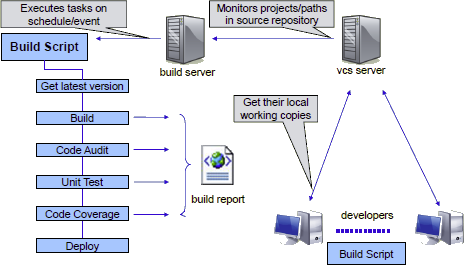
\includegraphics[scale=1.2]{umgebung_sw_konstruktion.png}
\end{center}
\pagebreak

\section{Konfigurations- und Versionsmanagement}
\subsection{Symptome von einem schlechten Versionsmanagement}
\begin{itemize}
 \item Alte Bugs tauchen wieder auf
 \item Alte Releases k\"onnen nicht gebuildet werden
 \item Alte Releases k\"onnen nicht gefunden werden
 \item Dateien gehen verloren
 \item Dateien sind pl\"otzlich ver\"andert
 \item Der selbe Code existiert in mehreren Projekten
 \item Zwei Entwickler arbeiten an Datei
\end{itemize}

\subsection{Versionsmanagement der Dateien}
\begin{tabular}{ll}
 \Bold{unter Versionsmanagement}&\Bold{nicht unter Versionsmanagement}\\
 $\bullet$ Sourcecode&$\bullet$ Alle generierten Dateien\\
 $\bullet$ Sourcefiles&$\bullet$ Generierte Javadoc\\
 $\bullet$ Konfigurationsdateien&$\bullet$ Binaries\\
 $\bullet$ Properties&$\bullet$ Log-Dateien\\
 $\bullet$ Build Files&$\bullet$ Testergebnisse\\
 $\bullet$ Ressourcen Files&\\
 $\bullet$ Benutzer-Doku&\\
\end{tabular}

\subsection{Versionsmanagement}
\begin{itemize}
 \item Repository: Datenbank, alle Dateien abgespeichert
 \item Working copy: Lokale Kopie
 \item Checkout: repo → working copy
 \item Commit: working copy → repo
 \item Update: Inline-Update
 \item Tagging: Snapshots vom Code\\
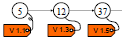
\includegraphics{tagging.png}
 \item Braching: Alternative Development-Version\\
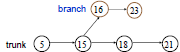
\includegraphics{branching.png}
\end{itemize}

\subsection{Bestandteile eines Konfigurationsmanagement}
\begin{itemize}
 \item Versions- und Releasemanagement
 \item Systembuilding (Tools wie ANT)
 \item Änderungsmanagement
 \item Planung von Konfigurationsmanagement
\end{itemize}

\subsection{Nummerierung von Revisionen}
\begin{enumerate}
 \item checkout
\begin{itemize}
 \item src/Main.java: 4
 \item src/Class.java: 4
 \item build/build.xml: 4
\end{itemize}
 \item Edit build.xml
\begin{itemize}
 \item src/Main.java: 4
 \item src/Class.java: 4
 \item build/build.xml: 8
\end{itemize}
 \item update
\begin{itemize}
 \item src/Main.java: 11
 \item src/Class.java: 11
 \item build/build.xml: 11
\end{itemize}
\end{enumerate}

\subsection{Merging}
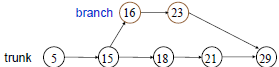
\includegraphics{merging.png}


\pagebreak
\section{Build Automation}
\subsection{Anforderungen f\"ur Build-Automation}
\begin{itemize}
 \item Build Server
 \item Versionsmanagement
 \item Tools
 \item Vor Ende des Tages eingecheckter Code
 \item Build-f\"ahriger Code
 \item Unit-Tests
\end{itemize}

\subsection{Visualisierung Build-Automation}
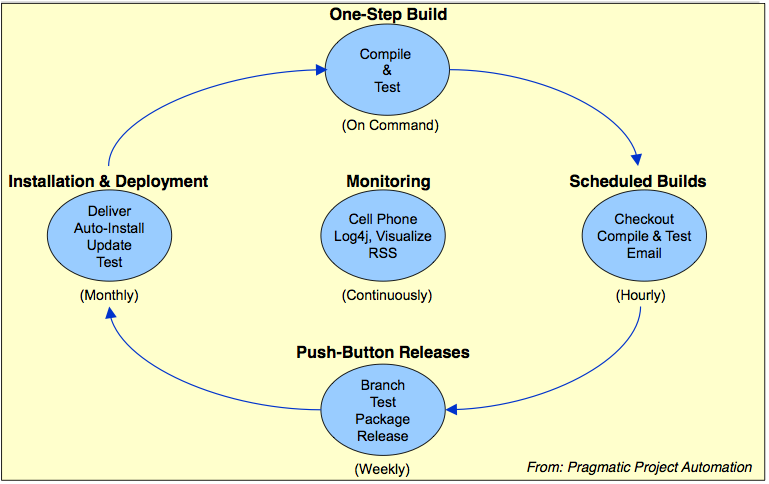
\includegraphics[scale=0.6]{build_automation.png}

\subsection{CRISP Builds}
\begin{itemize}
	\item[\Bold {Complete}] Alle dazugeh\"origen Ressourcen inbegriffen
	\item[\Bold {Repeatable}] Beliebig vielmal wiederholbar
	\item[\Bold {Informative}] Stellt wichtige Informationen bereit
	\item[\Bold {Schedulable}] Komplett und wiederholbar
	\item[\Bold {Portable}] Unabh\"angig von Maschine
\end{itemize}

\subsection{Ant-Script}
\lstinputlisting[language=Octave, label=Ant script, caption=Ant Script 1,style=MyAntStyle]{ant-script.xml}
\begin{lstlisting}[language=Octave, label=Ant script, caption=Ant Script 2a, style=MyAntStyle]
<target name="junitreport">
    <junitreport todir="${report.dir}">
        <fileset dir="${report.dir}" includes="TEST-*.xml"/>
        <report todir="${report.dir}"/>
    </junitreport>
</target>
\end{lstlisting}
\begin{lstlisting}[language=Octave, label=Ant script, caption=Ant Script 2b, style=MyAntStyle]
<path id="application" location="${jar.dir}/${ant.project.name}.jar"/>
<target name="run" depends="jar">
    <java fork="true" classname="${main-class}">
        <classpath>
            <path refid="classpath"/>
            <path refid="application"/>
        </classpath>
    </java>
</target>
\end{lstlisting}
\begin{lstlisting}[language=Octave, label=Ant script, caption=Ant Script 2c, style=MyAntStyle]
 <project name="MyProject" default="dist" basedir=".">
    <description>
        simple example build file
    </description>
  <!-- set global properties for this build -->
  <property name="src" location="src"/>
  <property name="build" location="build"/>
  <property name="dist"  location="dist"/>

  <target name="init">
    <!-- Create the time stamp -->
    <tstamp/>
    <!-- Create the build directory structure used by compile -->
    <mkdir dir="${build}"/>
  </target>

  <target name="compile" depends="init"
        description="compile the source " >
    <!-- Compile the java code from ${src} into ${build} -->
    <javac srcdir="${src}" destdir="${build}"/>
  </target>

  <target name="dist" depends="compile"
        description="generate the distribution" >
    <!-- Create the distribution directory -->
    <mkdir dir="${dist}/lib"/>

    <!-- Put everything in ${build} into the MyProject-${DSTAMP}.jar file -->
    <jar jarfile="${dist}/lib/MyProject-${DSTAMP}.jar" basedir="${build}"/>
  </target>

  <target name="clean"
        description="clean up" >
    <!-- Delete the ${build} and ${dist} directory trees -->
    <delete dir="${build}"/>
    <delete dir="${dist}"/>
  </target>
</project>
\end{lstlisting}


\newpage
\section{Continuous Integration}
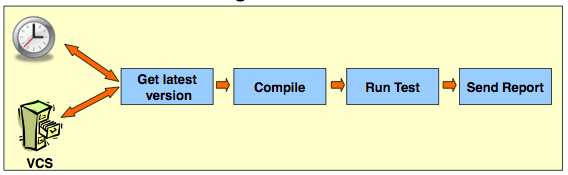
\includegraphics[scale=0.8]{continuous_integration.png}
\subsection{Vorteile}
\begin{itemize}
 \item Teamzusammenarbeit
 \item Komplexe Systeme werden managebar
 \item Reduziertes Risiko
 \item Module werden gezwungen, zusammenzuarbeiten
 \item Automatisches compile, run, testing und deploy
 \item Frühes Identifizieren von Problemen
 \item Immer einen deploy-f\"ahigen Build haben
 \item Immer Klarheit \"Uber den Status des Projekts haben
 \item Weniger Zeit in anspruch genommen um Fehler zu finden
 \item Weniger Zeit verschwendet wegen \"{ }broken code\"{ }
 \item Codequalit\"at verbessern mit hinzugef\"zgten Tasks
 \item Potenzielle Deploymentprobleme fr\"uhzeitig feststellen
\end{itemize}

\subsection{Nachteile}
\begin{itemize}
 \item Schwierig ein bereits vorhandenes Projekt in ein CI zu importieren
 \item Systeme die Serverkomponenten benutzen
 \item DB-basierte Systeme m\"ussen up-to-date sein
\end{itemize}


\subsection{Integration ist defekt wenn...}
\begin{itemize}
 \item Build nicht erfolgreich
 \item Gesharte Komponenten funktionieren nicht \"uberall gleich
 \item Unit-Tests nicht erfolgreich
 \item Code-Qualit\"at schlecht (Conventions, Metrics)
 \item Deployment nicht erfolgreich
\end{itemize}

\subsection{Anwendung von CI}
\begin{itemize}
 \item Ein einzelnes Code-Repo
 \item Build automatisieren
 \item Build testet automatisch
 \item Jeder commitet jeden Tag
 \item Jeder Commit sollte volle CI ausf\"uhren
 \item Testen in Klon von produktiver Umgebung
 \item Jeder hat den \"uberblick
 \item Automatisches Deployment
 \item Keep the build fast
 \item Jeder kann die neuste Version leicht erhalten
\end{itemize}

\subsection{Agiler Prozess}
\begin{itemize}
 \item Iterative Releases
 \item Planen von Builds
 \item Inkrementelles Implementieren
 \item Task f\"ur Task implementieren und immer wieder refactoring betreiben
 \item Report
 \item Output von CI ernst nehmen und bei Fehler Report
\end{itemize}

\subsection{Jenkins}
\begin{itemize}
 \item Continuous Integration Server
 \item Building, testing, Code Coverage, Analyse, ...
 \item Detaillierter Output
 \item Schneller \"uberblick \"uber Builds
 \item Dashboard praktisch f\"ur mehre Projekte
 \item Viele Plugins
\end{itemize}

\pagebreak
\section{Unit Testing}

\subsection{Aspekte des Testings}
\begin{itemize}
 \item[\Bold {Validation:}] 		Ist das Produkt \"uberhaupt das, was gew\"unscht wurde? 
 \item[\Bold {Verifikation:}]		Ist das Produkt korrekt programmiert
 \item[\Bold {Regression:}]	Iteratives Wiederholen von Tests 
 \item[\Bold {Software Fault:}]	Statischer Defekt in der Software
 \item[\Bold {Software Error:}]	State der durch Fehlfunktion von Software erreicht wurde
 \item[\Bold {Software Failure:}] 	Software wiederspiegelt Requirements nicht
\end{itemize}

\subsection{Der Testprozess}
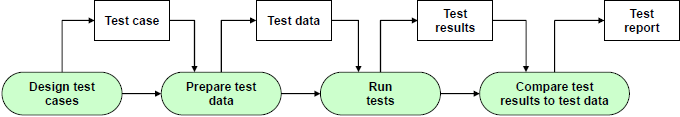
\includegraphics[scale=0.75]{unit_test.png}

\subsection{Gute Tests}
\begin{itemize}
	\item[\Bold {Automatic}] Tests ausf\"uhren und Resultate \"uberpr\"ufen
	\item[\Bold {Thorough}] Alles was fehlschlagen kann testen $\Ra$ Code coverage
	\item[\Bold {Repeatable}] Egal wieviel mal der Test gemacht wird, das Resultat ist das selbe
	\item[\Bold {Independent}] Test h\"angen nicht voneinander ab
	\item[\Bold {Professional}] gleicher professioneller Standard wie f\"ur den Code ben\"utzen
\end{itemize}

\subsection{Testdaten}
\subsubsection{Bestimmen von Testwerten:}
F\"{u}r die Rechnung $\sqrt{(X-1)\cdot(X+2)}\to$ Testet man die folgenden F\"{a}lle:
\begin{description}
\item[EC1] $X<=-2\to$ Valid
\item[EC2] $-2<X<1\to$ Invalid
\item[EC3] $X>=1\to$ Valid
\end{description}
Auch immer wichtig: Werte wie MAX\_$ $VALUE und MIN\_$ $VALUE nicht ausser Acht lassen
\subsubsection{Right-BICEP Testliste f\"{u}r Tests}
\begin{description}
\item [Right] Sind die Resultate richtig?
\item [B] Sind Randbedingungen (boundary) eingehalten worden?
\item [I]K\"{o}nnen inverse Beziehungen \"{u}berpr\"{u}ft werden?
\item [C] Sind die Resultate mit anderen Mittel cross-checked?
\item [E] Ist es m\"{o}glich, Error Conditions zu erzwingen?
\item [P]Stimmt die Performance?
\end{description}

\subsection{Test Klasse}
Die Test Klasse ist f\"{u}r das testen eines Elements verantwortlich
\begin{itemize}
	\item Deswegen ist normalerweise eine Test Klasse zum Testen einer einzigen Klasse zust\"{a}ndig
	\item Eine Test Klasse ist eine normale Java Klasse.
	\item Falls die Test Klasse im gleichen package, wie die zu testende Klasse ist, kann sie auf die default und protected Methoden zugreifen. Die Test Klassen sollten nicht im gleichen Source-Verzeichnis sein wie die zu testende Klasse.
\end{itemize}

\subsection{Begriffserkl\"{a}rung}
\begin{tabular}{lll}
CUT&\Bold {Class under Test}&Die zu testende Klasse\\
MUT&\Bold {Method under Test}&Die zu testende Methode\\
&\Bold {Test Case}&Spezifizierte Daten, um Methoden von CUT zu testen\\
&\Bold {Test Suite}&Mehrere Test Cases, f\"{u}r ein bestimmtes Ziel zust\"{a}ndig\\
&\Bold {Test Fixture}&Beispielsweise eine JUnit-Test-Klasse\\
\end{tabular}\\ \\
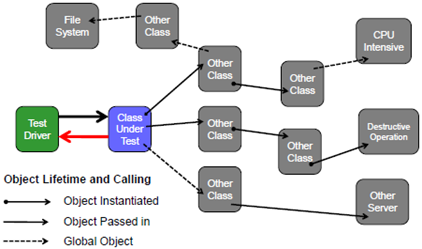
\includegraphics[scale=1]{Begriffe.png}

\subsection{HowTo}
\subsubsection{Set Up}
Um einen Test zu initialisieren, wird eine setup Methode, vor jeder Test Methode  aufgerufen
\begin{itemize}
	\item In der setup Methode die Testumgebung wird initialisiert
	\item Die setup Methode garantiert, dass jede Test Methode mit der gleichen Umgebung statt findet
	\item Eine setup Methode muss "public void" und ist mit @Before notiert sein 
\end{itemize}
\begin{lstlisting}[language=Java,caption=Unit Test (Before), style=MyJavaStyle]
@Before
public void setup() {
	... 
}
\end{lstlisting}

\subsubsection{Test Methode}
Eine Unittest Klasse besteht aus mehreren verschiedenen Test Methoden
\begin{itemize}
	\item Test bekommen kein Argument und geben nichts zur\"{u}ck
	\item Jede Test Methode sollte komplett unabh\"{a}ngig von anderen Test Methoden sein
	\item Meistens testet eine einzelne Test Klasse eine individuelle Methode von der zu testenden Klasse.
	\item Eine Test Methode muss "public void" und mit @Test notiert sein
\end{itemize}
\begin{lstlisting}[language=Java,caption=Unit Test (Test), style=MyJavaStyle]
@Test
public void testY() {
	... 
}
\end{lstlisting}

\subsubsection{Tear Down}
Nach jeder Test Methode wird eine tear down Methode aufgerufen
\begin{itemize}
	\item Die tear down Methode bringt alles wieder auf den letzten Stand.
	\item So kann ist jedes Ergebnis das selbe und es wird nicht von anderen Tests verf\"{a}lscht.
	\item Eine Test Methode muss \"{ }public void\"{ } und mit @After notiert sein
\end{itemize}
\begin{lstlisting}[language=Java,caption=Unit Test (After), style=MyJavaStyle]
@After
public void teardown() {
	... 
}
\end{lstlisting}

\subsubsection{Assertions}
Assertions werden zum Vergleichen von erwarteten Resultaten genutzt.
\begin{description}
	\item[assertEquals($<Type>$ expected, $<Type>$ actual)] \hfill
		\begin{itemize}
			\item Vergleicht primitive Typen am Wert
			\item Vergleicht Klassen Typen mit dem Aufruf equals
			\item \"{u}berladed mit allen primitiven Typen, Objekten und Strings.
		\end{itemize}
	\item[assertSame(Object expected, Object actual)] \hfill \\
		Vergleicht Referenzen mittels ==-Operator
	\item[assertNull(Object x), assertTrue(boolean b)] \hfill \\
	\item[fail()] \hfill \\
		L\"{a}sst den Test manuell failen
\end{description}

\subsubsection{Exception}
Exceptions k\"{o}nnen getested werden. Falls nur eine Exception erwartet wird:
\begin{itemize}
	\item Schreibe die Exception  zu einem expected Argument in der @Test Notation.
	\item @Test(expected=IllegalArgumentException.class)
\end{itemize}

\subsection{Beispiele}
\lstinputlisting[language=Java,caption=Unit-Test Beispiel,style=MyJavaStyle]{unit-test.java}

\pagebreak
\section{Isolated Testing}

\subsection{Test doubles in Unit Testing}
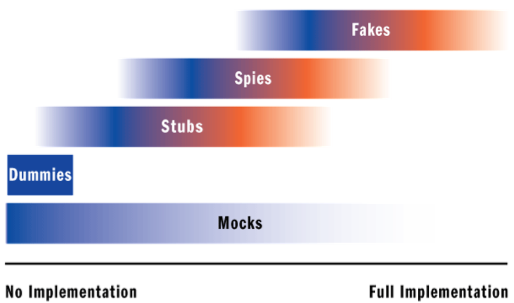
\includegraphics[scale=0.8]{test_doubles.png}
\begin{itemize}
	\item[\Bold {Dummy}] Meist nur benutzt, um Parameter-Listen zu f\"{u}llen 
	\item[\Bold {Stubs}] Minimale Implementation von Schnittstellen oder Basisklassen, void hat  normalerweise kein Code und die anderen Methoden fest kodierte Werte
	\item[\Bold {Spys}] \"{a}hnlich wie Stubs, aber zeichnen verwendete Mitglieder von Klasse auf
	\item[\Bold {Fakes}]Haben bereits oft komplexe Implementierung, managen Interaktion zwischen verschiedenen Mitglieder von denen sie erben
	\item[\Bold {Mocks}] Vorprogrammierte Objekte mit fest kodierten Erwartungen
\end{itemize}
\begin{lstlisting}[language=Java,caption=Beispiel von Stub, style=MyJavaStyle]
class EmailStub {
    void sentMail (String mailText) {
    ;
    }
}
\end{lstlisting}
Parameter\"{u}bergabe funktioniert, jedoch wird keine Funktion ausgef\"{u}hrt, da nur void.

\subsection{Mock Testing}
Mock-Objekte simulieren Teile des Verhaltens von Domain-Objekten. Klassen k\"{o}nnen in Isolation, durch die Simulation von ihren Mitarbeitern, mit Mock-Objekte getestet werden. Nimmt Klassen aus einer nat\"{u}rlichen Umgebung und stellt sie in einem gut definierte Testumgebung.

\subsubsection{Einsatzbereich von Mock-Objekten}
\begin{itemize}
	\item Verhalten von realem Objekt ist nicht-deterministisch
	\item Reale Objekt schwierig aufzusetzen
	\item Reale Objekt ist langsam
	\item Reale Objekt verf\"{u}gt \"{u}ber GUI
	\item Der Test muss das orginal Objekt fragen wie es war
	\item Reale Objekt existiert nicht nicht
\end{itemize}
\begin{description}
	\item[Pros] \hfill
		\begin{itemize}
			\item Test v\"{o}llig isoliert
			\item Vereinfacht Schnittstelle zu vielen Methoden
			\item Nahezu alles kann getestet werden wie z.B. JDBC
		\end{itemize}
	\item[Cons] \hfill
		\begin{itemize}
			\item Kann Implementierung zu \"{a}hnlich sein, k\"{o}nnte den Test unbrauchbar machen
			\item Kann komplex werden bei z.B. JDBC
		\end{itemize}
\end{description}

\subsection{EasyMock}

Generiert Mock Objekte dynamisch, es ist nicht n\"{o}tig, sie selbst zu schreiben und Code zu generieren.
\begin{itemize}
\item Kreieren
\item Aufzeichnen
\item Replay
\item Normales Testing
\item Verify
\end{itemize}

\subsubsection{Spezielle Vorteile von EasyMock}
\begin{itemize}
\item Selber-kodieren von Mock Objekten f\"{a}llt weg
\item Sind Refactor-Safe, wird also eine Methode umbenannt ist das kein Problem
\item Return Werte \& Exceptions sind unterst\"{u}tzt
\item Erlaubt \"{u}berpr\"{u}fung der Reihenfolge, in welcher Methoden aufgerufen werden vom Mock Objekt
\item Anzahl der Aufrufe einer Mock-Objekts k\"{o}nnen \"{u}berwacht werden
\end{itemize}

\subsubsection{Ablauf}
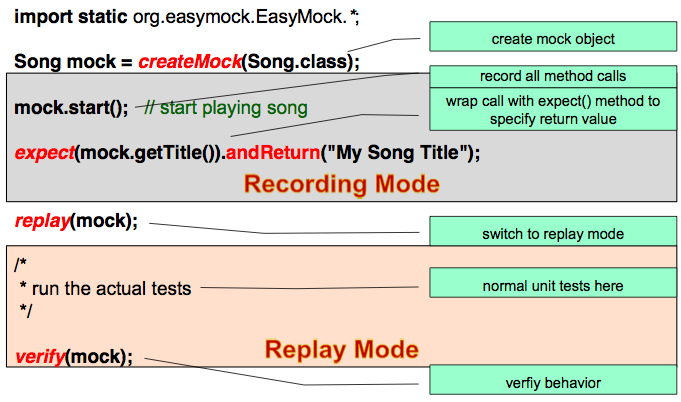
\includegraphics[scale=0.6]{easymock.png} \\

\subsubsection{Befehle}
\begin{description}
	\item[createMock(Class$<T>$ toMock)] \hfill \\
		Creates a mock object that implements the given interface, order checking is disabled by default.
	\item[createStrictMock(Class$<T>$ toMock)] \hfill \\
		Creates a mock object that implements the given interface, order checking is enabled by default.
	\item[createNiceMock(Class$<T>$ toMock)] \hfill \\
		Creates a mock object that implements the given interface, order checking is disabled by default, and the mock object will return 0, null or false for unexpected invocations.
	\item[expect$<T>$(T value)] \hfill \\
		Returns the expectation setter for the last expected invocation in the current thread.
	\item[expectLastCall()] \hfill \\
		Returns the expectation setter for the last expected invocation in the current thread. This method is used for expected invocations on void methods. 
	\item[reset()] \hfill \\
		Resets the given mock objects (more exactly: the controls of the mock objects).
	\item[replay()] \hfill \\
		 Switches the given mock objects (more exactly: the controls of the mock objects) to replay mode.
	\item[verify()] \hfill \\
		Verifies the given mock objects (more exactly: the controls of the mock objects).	 
	\item[andThrow(jThrowable)] \hfill \\
		Sets a throwable that will be thrown for the expected invocation.
	\item[times(count), times(min, max), once(), atLeastOnce() \& anyTimes()] \hfill \\
		Those defines number of expected calls.
\end{description}
\subsubsection{Beispiel}
\lstinputlisting[label=Mock-Test,caption=Beispiel Mock-Test1, style=MyJavaStyle]{mock-test.java}


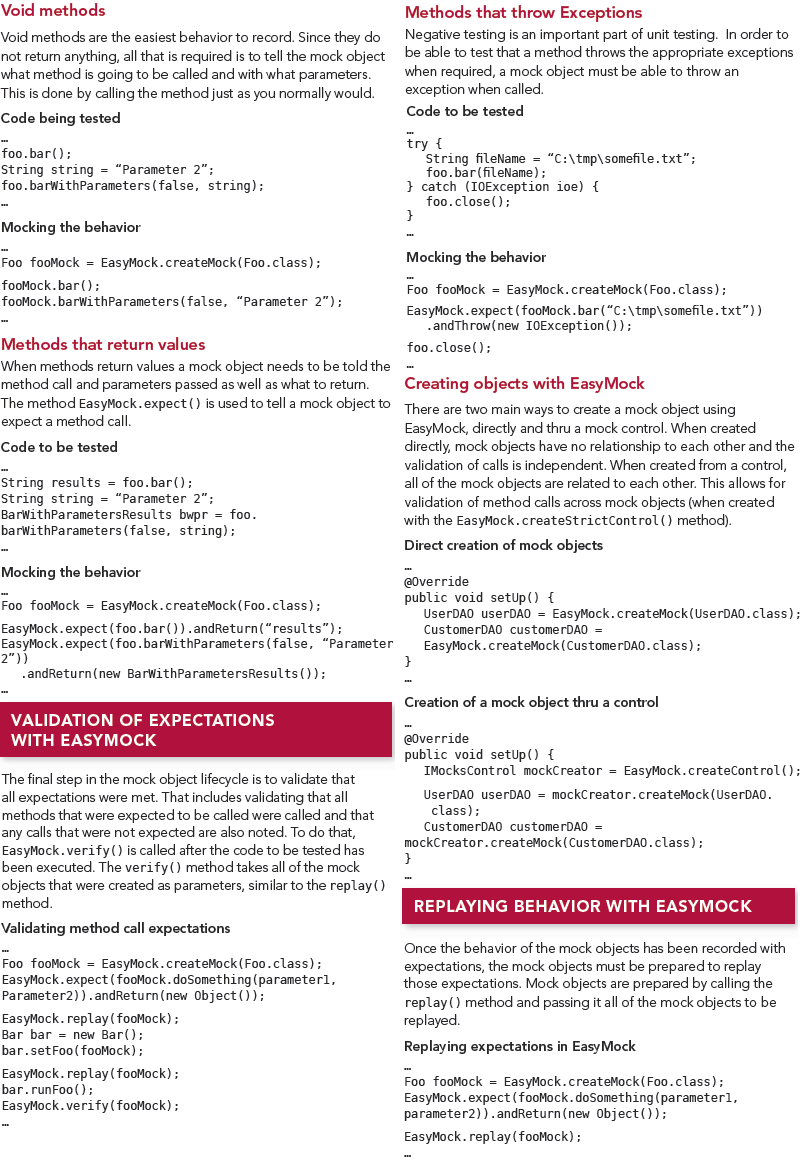
\includegraphics[scale=0.8]{EasyMockStuff.png}

\pagebreak
\section{Software Quality Metrics}
\subsection{Was ist Software Qualit\"{a}t?}
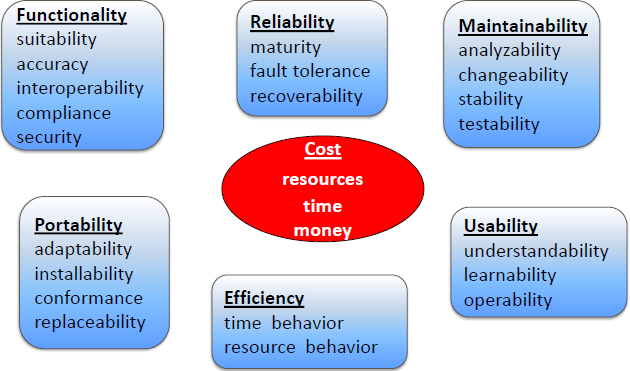
\includegraphics[scale=1]{Metrics.png}
\subsection{Metric (Def)}
\begin{description}
	\item[Size Metrics] \hfill 
		\begin{itemize}
			\item Lines of Code(LoC)
			\item Number of Statements
			\item Fields, Methods
			\item Packages
		\end{itemize}
	\item[Dataflow Metrics] \hfill
		\begin{itemize}
			\item Cyclomatic Complexity (McCabe Complexity)
			\item Dead Code detection
			\item Initialization before use
		\end{itemize}
	\item[Style Metrics] \hfill 
		\begin{itemize}
			\item Number of Levels (nesting depth)
			\item Naming conventions, formatting conventions
		\end{itemize}
	\item[OO Metrics] \hfill
		\begin{itemize}
			\item No. of classes, packages, methods
			\item Inheritance depth / width
		\end{itemize}
	\item[Coupling Metrics] \hfill
		\begin{itemize}
			\item LCOM: lack of cohesion metrics
			\item No. of calling classes / no. of called classes
			\item Efferent / Afferent couplings
		\end{itemize}
	\item[Statistic Metrics] \hfill
		\begin{itemize}
			\item Instability
			\item Abstractness
		\end{itemize}
	\item[Performance Metrics (dynamic)] \hfill 
		\begin{itemize}
			\item Time spent
			\item Memory consumption (also memory leaks)
			\item Network traffic
			\item Bandwidth needed
			\item No. of clicks to perform a task
		\end{itemize}
	\item[Other dynamic metrics] \hfill 
		\begin{itemize}
			\item No. of tests executed
			\item No. of failed tests
			\item Code coverage
		\end{itemize}
\end{description}

\subsection{Cyclomatic Complexity}
Anzahl von m\"{o}glichen verschiedenen Pfaden durch den Code. So wird gerechnet:
Cyc. Complex. $= b + 1$, wobei $b =$ bin\"{a}re Entscheidungen wie \Bold {if, while, for, case,} ...\\
$N < 10 \Ra $ code ist gut lesbar\\
Kritik: switch ist gut lesbar aber treibt die Cyclomatic Complexity nach oben

\subsection{Cohesion and Coupling Metrics}
\begin{description}
	\item[Cohesion] \hfill \\
		Misst, wie nahe sich die Klassen sind
	\item[Coupling / Dependency] \hfill \\
		Misst den Grad, wie fest Klasse von anderen abh\"{a}ngig
	\item Tiefe coupling normalerweise korreliert mit hoher cohesion
	\item Metrics: LCOM (Lack of Cohesion in Method)
\end{description}

\subsubsection{LCOM}
$LCOM^{HS} = \frac{m-avg(r(f))}{m}$
\begin{description}
	\item[Where] \hfill
		\begin{itemize}
			\item m is the number of methods of a class
			\item r(f) is the number of methods that access a field f
			\item Average r(f) over all fields.
		\end{itemize}
	\item[Examples] \hfill
		\begin{itemize}
			\item Each method accesses only one field \\
				$LCOM^{HS}$ = (almost) 1 low cohesion \\
				$\ra$ i.e. getters/setters are bad
			\item Each method reads all fields \\
				$LCOM^{HS}$ = 0 high cohesion
		\end{itemize}
\end{description}

\subsubsection{Emma Features (Java-Code-Coverage Instrument)}
\begin{itemize}
\item Byte Code und Offline and on-the-fly
\item \"{u}berpr\"{u}ft Klassen, Methoden, Linien und Standardbl\"{o}cke
\item Reportet in TXT, HTML, XML
\item Statistik m\"{o}glich \"{u}ber Methode, Klasse, Package oder alle Klassen
\item Ausf\"{u}hrbar via ANT, CMD, Eclipse Plugin
\end{itemize}

\subsubsection{Warum Metrics verwenden?}
\begin{itemize}
\item Wichtiges Tool f\"{u}r Qualit\"{a}tsmessung
\item �You can't manage what you can't control, and you can't control what you don't measure�
\item Jedoch nicht \"{u}bertreiben mit Messen, ein sinnvolles Mass soll gefunden werden
\end{itemize}


\pagebreak
\section{Refactoring}
\begin{itemize}
	\item Refactoring verbessert das Design Ihres Systems
	\item Refactoring macht Ihre Software einfacher zu verstehen
	\item Refactoring hilft Ihnen, Fehler zu finden
\end{itemize}
\Bold {Versuche nicht, Features hinzuzuf\"{u}gen, wenn man den  Refactoring-Hut tr\"{a}gt.} \\ \\
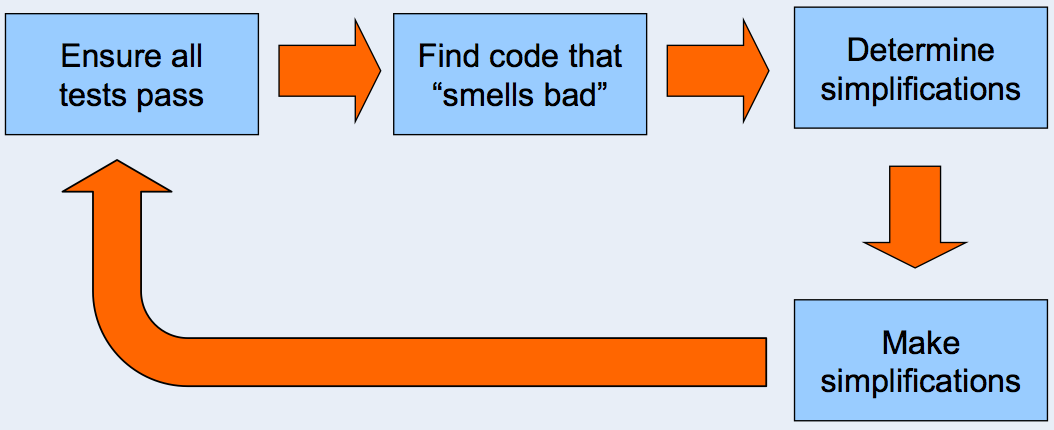
\includegraphics[scale=0.4]{refactoring_workflow.png}

\subsection{Problems}
\begin{itemize}
	\item Zu weit getrieben, kann Refactoring zu unaufh\"{o}rliche Bastelei mit dem Code f\"{u}hren, damit es perfekt wird.
	\item Datenbanken k\"{o}nnen schwierig sein zu refactoren sein
	\item Refactoring ver\"{o}ffentlicht Schnittstellen k\"{o}nnen Probleme f\"{u}r den Code bringen, die diese Schnittstellen ben\"{u}tzen
\end{itemize}

\subsection{Code Smells}
\begin{description}
	\item[Too Much Code Smells] \hfill
		\begin{itemize}
			\item Doppelter Code
			\item Lange Methoden
			\item Grosse Klassen
			\item Lange Parameter Listen
			\item Feature Envy
			\item Switch Statements
			\item Parallele Vererbungshierarchie
		\end{itemize}
	\item[Not enough� Code Smells] \hfill 
		\begin{itemize}
			\item Leere Catch clause
		\end{itemize}
	\item[Code Change Smells] \hfill
		\begin{itemize}
			\item Divergent Change
			\item Shotgun Surgery	
		\end{itemize}
	\item[Comment Smells] \hfill 
		\begin{itemize}
			\item Muss kommentiert werden
			\item Zu viel Kommentar
		\end{itemize}
\end{description}

\subsection{How To}
\subsubsection{Extract Method}
Code-Fragmente in eigene Methoden fassen. Grosse Methoden in kleine aufteilen.\\
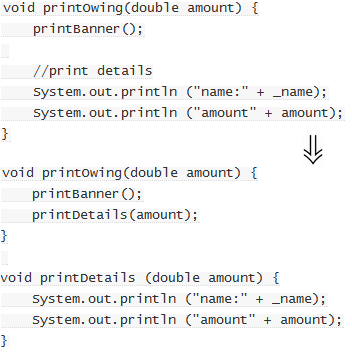
\includegraphics[scale=.6]{refactoring_1.png}
\subsubsection{Self Encapsulate Field}
Getter- und Setter-Methoden einsetzen. Damit ist ein einheitlicher Zugriff von aussen sichergestellt, unabh\"{a}ngig ob das Resultat aus einer Variable oder Berechnung stammt.\\
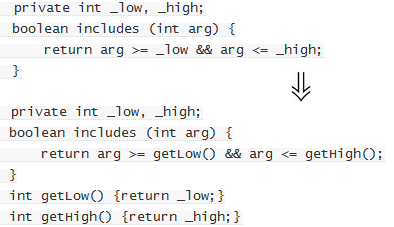
\includegraphics[scale=.6]{refactoring_2.png}
\subsubsection{Move Method}
Wenn eine Methode mehr auf Daten einer fremden Klasse als auf die der eigenen Klasse zugreift, ist sie ein guter Kandidat um in die andere Klasse verschoben zu werden.\\
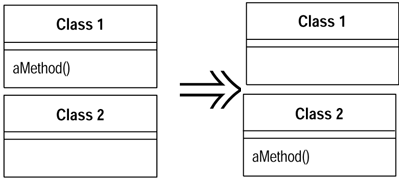
\includegraphics[scale=.6]{refactoring_3.png}
\subsubsection{Replace Temp with Query}
Komplizierte Berechnungen in eigene Methoden verschieben, anstatt deren Resultat in Variablen zu speichern.\\
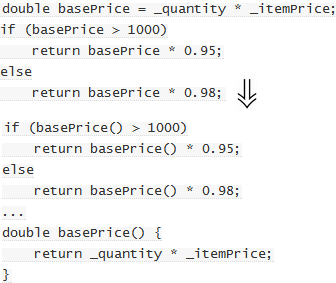
\includegraphics[scale=.6]{refactoring_4.png}
\subsubsection{Replace Type Code with State/Strategy}
Eine Klasse hat verschiedene Verhaltensweisen abh\"{a}ngig von einer Typ- oder Statusvariable. Verwendung des Strategy- oder State-Patterns (Aggregation einer abstrakten Klasse mit entsprechenden Unterklassen) um verschiedene F\"{a}lle mit Polymorphie abzufangen.\\
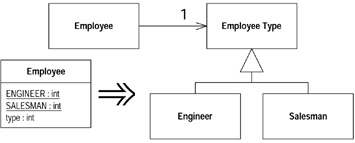
\includegraphics[scale=.6]{refactoring_5.png}
\subsubsection{Replace Conditional with Polymorphism}
Ebenfalls Verwendung von Polymorphie. Jeder Fall eines Case-Statements wird in eine eigene Unterklasse verschoben.\\
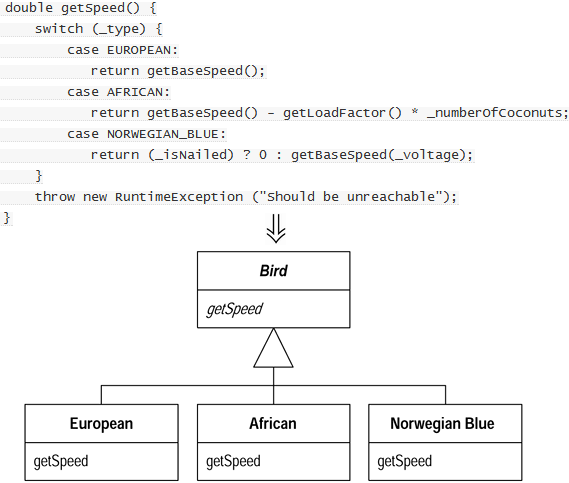
\includegraphics[scale=.6]{refactoring_6.png}

\pagebreak
\section{Coding Style \& Clean Code}
Sauberer Code ist einfach und direkt. Sauberer Code liest sich wie gut geschriebene Prosa. Sauberer Code niemals verdeckt die Absicht des Konstrukteurs, sondern ist voll von frischen Abstraktionen und einfache Linien der Kontrolle. \\
\subsection{Warum soll man Code Conventions befolgen?}
\begin{itemize}
\item 80\% der Lebensdauer einer Software besteht aus Wartung
\item Kaum eine Software wird nur vom Autor gewartet
\item Verbessern Lesbarkeit, so dass neuer Code schneller und besser zu verstehen ist
\item Macht Code einfacher zu verbessern und Bugs zu entdecken
\end{itemize}
Code conventions denkt die folgenden Themen ab: 
\begin{description}
	\item[Dateinamen und -organisation] \hfill 
		\begin{itemize}
			\item Dateinamen, Ordner
			\item Ordnerstruktur eines Projekts
			\item Struktur der Codedateien
		\end{itemize}
	\item[Einr\"{u}ckung] \hfill
		\begin{itemize}
			\item Tabs vs. Leerschl\"{a}ge
			\item Linienl\"{a}nge
			\item Linienumbruch, Zeilenumbruch Regeln
		\end{itemize}
	\item[Namenskonventionen] \hfill
		\begin{itemize}
			\item Namenskonventionen machen Programme verst\"{a}ndlicher, so dass sie leichter zu lesen, zu verbessern und um Fehler zu erkennen
		\end{itemize}
	\item[Erkl\"{a}rungen, \"{a}usserungen und White Spaces] \hfill 
		\begin{itemize}
			\item Wie viele Variablendeklarationen pro Linie?
			\item Wo sollen Variablen deklariert werden?
			\item Wo sollen die \}\} Klammern sein?
			\item Wo sollen leere Linien sein?
		\end{itemize}
\end{description}

\subsection{API Documentation}
API-Dokumentation ist ein Vertrag zwischen Ihnen und den Kunden von Ihrem Code. Es gibt den Zweck der Klasse / Interface und die Funktionalit\"{a}t der Methoden. Biete was wirklich gebraucht wird.

\subsection{Klassen/Interface Dokumentation}
\begin{itemize}
	\item Spezifiziert Sinn und Zust\"{a}ndigkeit von Klasse, wenn m\"{o}glich in 1 Satz
	\item Spezifiziert wichtige Eigenschaften, die nicht durch Code ausgedr\"{u}ckt sind
	\item Klasse: Erkl\"{a}rt Eigenschaft verwendete Algorithmen (Performance, Speicher, �)
	\item Interface: Erkl\"{a}rt, was gemacht wurde und nicht wie es gemacht werden soll
\end{itemize}

\subsection{Methoden Dokumentation}
\begin{itemize}
	\item Spezifiziert was man vom Aufrufer erwartet (Percond., Parameter)
	\item Spezifiziert was man dem Aufrufer zur\"{u}ckgibt (Postcond., Invariante., Return-Wert)
\end{itemize}

\subsection{Wichtig zu beachten}
\begin{itemize}
\item Selbstsprechende Namen sind sehr wichtig und sollen gebraucht werden
\item Mittels TODO, FIXME (Bug) und XXX (Nochmals \"{u}berdenken) k\"{o}nnen Marker gesetzt werden, Eclipse unterst\"{u}tzt dies und zeigt diese an
\end{itemize}

\subsection{JavaDoc}
Javadoc ist ein separates Programm, das mit dem JDK mitgeliefertwird. Es liest das Programm, macht Listen aller Klassen, Interfaces, Methoden und Variablen, und erzeugt HTML-Seiten auf der die Ergebnisse angezeigt werden. \\
Schreibe Kommentare f\"{u}r den Programmierer der die Klasse ben\"{u}tzt: 
\begin{itemize}
	\item Alles, was man ausserhalb der Klasse zur Verf\"{u}gung stellen will, sollten dokumentiert werden
	\item Es ist eine gute Idee, private Elemente  ,f\"{u}r den eigenen Gebrauch, zu beschreiben
\end{itemize}
javadoc kann Dokumentation erzeugen f\"{u}r:
\begin{itemize}
	\item nur public Elemente
	\item public und protected Elemente
	\item public, protected, und package Elemente
	\item alle die public, protected, package, and private Elemente sind
\end{itemize}
JavaDoc ist m\"{o}glich bei:
\begin{itemize}
	\item Package
	\item Klasse
	\item Interface
	\item Konstruktor
	\item Methode	
	\item Feld
\end{itemize}

\subsubsection{Tags In javadoc Comments}
\begin{description}
	\item[@param p] Beschreibung von Parameter p.
	\item[@return] Beschreibung des return values (ausser die Method returns void).
	\item[@exception e] Beschreibe eine beliebige Exception.
	\item[@see] F\"{u}gt ein "See Also" hinzu mit einem Link oder text das auf eine Referenz zeigt
	\item[@author] dein Name
	\item[@version] eine Versionsnummer oder -datum
\end{description}

\subsection{Programming Practices}
\begin{itemize}
\item Keine �magischen Zahlen� wie 4.352, viel besser Konstanten verwenden
\item Run-Time Performance verbessern sollte man dem Compiler \"{u}berlassen
\item Kein if (value == true) { return true; } else { return false; } $\to$ return value;
\item In einer Methode nur etwas machen und nicht mehre Sachen
\item If (!value) ist nicht so gut lesbar wie if (value)
\end{itemize}

\subsection{Checkstyle}
\begin{itemize}
\item \"{u}berpr\"{u}ft Code nach vorgegebenen Regeln
\item Eigene Tests k\"{o}nnen geschrieben werden
\item XML-Konfigurationsdatei wird verwendet
\end{itemize}

\begin{lstlisting}[language=Java,caption=JavaDoc Beispiel 1, style=MyJavaStyle]
/**
 * Manages the stock of videos of the rental shop.
 * @author Christoph Denzler
 *
 */
public class Stock {
  
  /** The stock of videos. */
  private HashMap<String, Integer> stock = new HashMap<String, Integer>();
  
  /** low stock listeners. */
  private List<LowStockListener> listeners = new LinkedList<LowStockListener>();
  
  /**
   * add a movie to the stock.
   * @param movie the movie to add to the stock.
   * @return the number of items of this movie in stock after this operation.
   */
  public int addToStock(IMovie movie) {
\end{lstlisting}

\begin{lstlisting}[language=Java,caption=JavaDoc Beispiel 2, style=MyJavaStyle]
    /**
     * Create a new user with the given name information.
     * 
     * @param aName the user's family name.
     * @param aFirstName the user's first name.
     * @param aBirthdate the user's birth date.
     * @throws NullPointerException The name must neither be <code>null</code>.
     * @throws MovieRentalException If the name is empty ("") or longer than 40 characters.
     */
\end{lstlisting}

\begin{lstlisting}[language=Java,caption=JavaDoc Beispiel 3, style=MyJavaStyle]
    /**
     * The first three days cost only 1.5, then each days costs an extra 1.5.
     * 
     * @see ch.fhnw.edu.rental.model.PriceCategory#getCharge(int)
     * @param daysRented no of days that a movie is rented.
     * @return rental price for movie.
     */
    @Override
    public double getCharge(int daysRented) {
\end{lstlisting}

\pagebreak
\section{Logging}
\begin{itemize}
	\item Wichtig f\"{u}r Monitoring und Debugging Applikationen
\item Debugging: Interessiert den Status des Programmes  im Zeitpunkt des Ausf\"{u}hrens
\item Logging: Stellt Logging-Daten \"{u}ber ein Programm \"{u}ber eine Zeitspanne bereit
\item Wichtig bei Echtzeit-Systemen, verteilten Systemen und gleichzeitige Systeme
\end{itemize}

\subsection{Vorteile}
\begin{itemize}
	\item Die Konfiguration der Logging-Funktionen wird ausgelagert
	\item Log Nachrichten k\"{o}nnen priorisiert werden
	\item Logging unterst\"{u}tzt verschiedene Nachrichtsformatierungen
	\item An und Abschalten w\"{a}hrend das Programm l\"{a}uft
	\item Unterst\"{u}tzt verschiedene Ausgabe Ziele
	\item Verschiedene Ausgabe Stufen
	\item Unterst\"{u}tzt Nachtrichten abfangen um Performanz hoch zu halten
\end{itemize}

\subsection{Log4j}
\begin{itemize}
\item Soll verwendet werden und nicht System.out.println
\item Output kann extern ausgegeben werden, Priorisierung, versch. Ausgabeformate, zur Laufzeit aktiviert bzw. deaktiviert werden, verschiedene Logstufen, Message-Caching wird unterst\"{u}tzt, um Performance-Einbusse zu verhindern
\end{itemize}

\subsection{Konzept}
\begin{itemize}
	\item[\Bold {Priority}] Bestimmt, was geloggt wird.
	\item[\Bold {Level}] Bestimmt, ob etwas geloggt wird.
	\item[\Bold {Appender}] Bestimmt, wo etwas geloggt wird.
	\item[\Bold {Layout}] Bestimmt, wie das Layout aussieht.
	\item[\Bold {Logger}] Schreibt einen Log-Eintrag zu einem Appender in einem bestimmten Layout falls das Logginglevel angemessen ist.
\end{itemize}

\subsection{Logging Levels}
\begin{itemize}
	\item[\Bold {FATAL}] Fehler, bei dem die Applikation sich nicht mehr erholen kann
	\item[\Bold {ERROR}] Fehler, die Applikation ist jedoch nicht lauff\"{a}hig
	\item[\Bold {WARN}] Informiert \"{u}ber �schlimmes� Ereignis
	\item[\Bold {INFO}] Informiert z.B. \"{u}ber Fortschritt der Applikation
	\item[\Bold {DEBUG}] Stellt Informationen f\"{u}r Debug bereit 
	\item[\Bold {TRACE}] Sehr detaillierte Informationen um Informationsfluss zu verfolgen
Werden direkt auch so aufgerufen $\to$ info(Object message [, Throwable throwable] ); oder log(Priority level, Object message,Throwable throwable);
\end{itemize}

\subsection{Aufbau des Loggers}
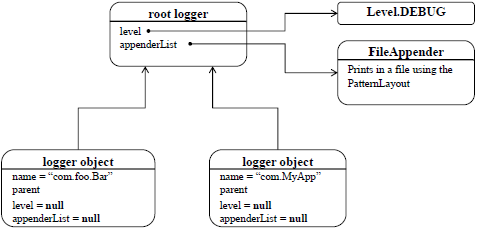
\includegraphics[scale=1]{log4j.png}

\subsection{Verschiedene Appender}
\begin{itemize}
\item ConsoleAppender - Write log to System.out or System.err
\item FileAppender � Write to a log file
\item SocketAppender � Dumps log output to a socket
\item SyslogAppender � Write to the syslog.
\item NTEventLogAppender � Write the logs to the NT Event Log system.
\item RollingFileAppender � After a certain size is reached it will rename the old file and start with a new one.
\item SocketAppender � Dumps log output to a socket
\item SMTPAppender � Send Messages to email
\item JMSAppender � Sends messages using Java Messaging Service
\end{itemize}

\subsection{PatternLayout Platzhalter}
\begin{itemize}
\item[\Bold{\%C:}] For example, for the class name org.apache.xyz.SomeClass, the pattern \%C{1} will output SomeClass
\item[\Bold{\%d}]: For example, \%d\{HH:mm:ss,SSS\} or \%d\{dd MMM yyyy HH:mm:ss,SSS\}
\item[\Bold{\%F:}] Datei, die das Logging veranlasst hat
\item[\Bold{\%L:}] Code-Linie vom Logevent
\item[\Bold{\%m:}] Message
\item[\Bold{\%M:}] Methode
\item[\Bold{\%n:}] Neue Linie wie �$\backslash$n�
\item[\Bold{\%p:}] Priorit\"{a}t
\item[\Bold{\%r:}] Zeitmessung Logevent
\item[\Bold{\%t:}] Thread
\end{itemize}

\subsection{Best Practices} 
\begin{itemize}
\item e.printStackTrace() nicht verwenden sondern log.error("Exception message", e)
\item Keine Exception loggen und sie dann trotzdem werfen
\item Wenn m\"{o}glich immer Stack Trace anh\"{a}ngen mit \} catch(SQLException e)\{ 
throw new RuntimeException("DB exception", e); \}
\end{itemize}

\lstinputlisting[language=Octave,caption=Log4j XML Teil,style=MyAntStyle]{log4j.xml}
\lstinputlisting[language=java,caption=Log4j Java Teil,style=MyJavaStyle]{log4j.java}


\pagebreak
\section{GUI- Testing}
\subsection{Zweck von GUI Tests test?}
\begin{itemize}
\item Werden richtige Funktionen ausgef\"{u}hrt?
\item Wird die Funktion korrekt ausgef\"{u}hrt?
\item Ist der Navigationsfluss korrekt?
\item Stellt das GUI die Daten korrekt dar?
\item Zeigt das GUI die richtigen Daten?
\item Sind die Steuerungen im richtigen Zustand?
\end{itemize}

\subsection{How to GUI-Testing}
\subsubsection{Manuall}
\begin{itemize}
\item Jeder Schritt wird von Hand ausgef\"{u}hrt.
\item Sehr arbeitsintensiv, sehr fehleranf\"{a}llig.
\item Muss jedes Mal erneuert werden, falls ein Regressionstests erforderlich ist.
\item Sehr teuer
\end{itemize}
Es ist schwierig ein manueller Test systematisch zu handhaben.

\subsubsection{Capture / Replay}
\begin{itemize}
\item Meist mehrere Prorgamme, die Benutzereingaben aufzeichnen
\item Umfasst meistens Scripting
\item Grosser Nachteil: \"{a}ndert GUI muss auch Test neu gemacht werden
\end{itemize}


\subsubsection{Scripting - In a seperate scripting language}
\textbf{\Bold Workflow:} $Writing Script \Longrightarrow SCRIPT \Longrightarrow REPLAY TOOL \Longrightarrow Execute Tests Automatically$

\begin{itemize}
\item Weitere Programmiersprache
\item Muss an irgendeiner Form der formalen Verifikation unterzogen werden.
\item Eliminiert menschliche Fehler w\"{a}hrend der Ausf\"{u}hrung des Tests.
\item Kann f\"{u}r Regressionstests benutzt werden (manchmal auch mit Modifikationen).
\item Verschiedene Ans\"{a}tze zum Testen.
\item Spion GUI Steuerung.
\item Bildverarbeitung
\end{itemize}

\subsubsection{Integrated Test Framework (Unit Test Programming Style)}
\begin{itemize}
\item Scripting braucht selbe Programmiersprache wie prod. Code
\item Scripts einfach/schnell anpassbar und vollst\"{a}ndig in DIE integriert
\item Wird meistens gleichzeitig wie Unit-Tests ausgef\"{u}hrt
\item Wichtige Aspekte f\"{u}r Test-Driven Development
\begin{itemize}
\item Model von der View trennen (siehe MVC-Modell)
\item Eindeutige Namen f\"{u}r jedes GUI-Element
\item Nicht zu �tief� testen, wie z.B. Verhalten von Standardkomponenten
\item Fokus auf Pr\"{u}fung des Verhaltens/Zustandes des GUIs
\end{itemize}
\end{itemize}

\subsection{FEST (GUI-Testing Tool)}
\begin{itemize}
\item A Collection of API's for functional Swing GUI testing
\item Simulation of user-generated events and reliable GUI component lookup
\item Easy-to-use and powerful API that simplifies creation and maintenance of Swing GUI functional tests
\item Runs JUnit or TestNG test
\end{itemize}

\subsubsection{Workflow}
\begin{enumerate}
\item Create a setup method to create your own GUI instance (either frame or dialog)\\
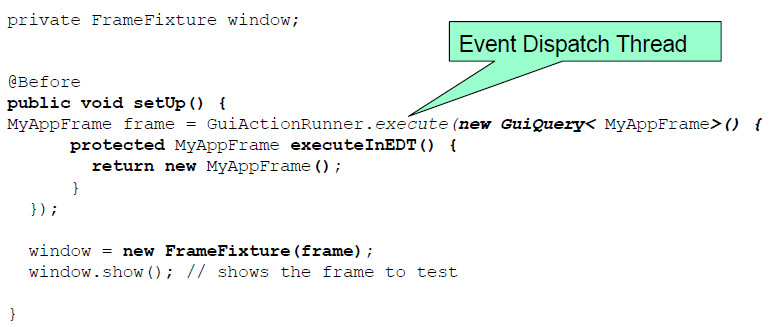
\includegraphics[scale=0.6]{FEST_Setup.png}

\item Close window and release resources\\
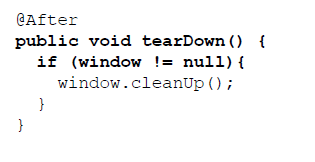
\includegraphics[scale=0.6]{FEST_CleanUP.png}
\pagebreak
\item Execute the actions on the controls
\item Verify expected behavior.\\
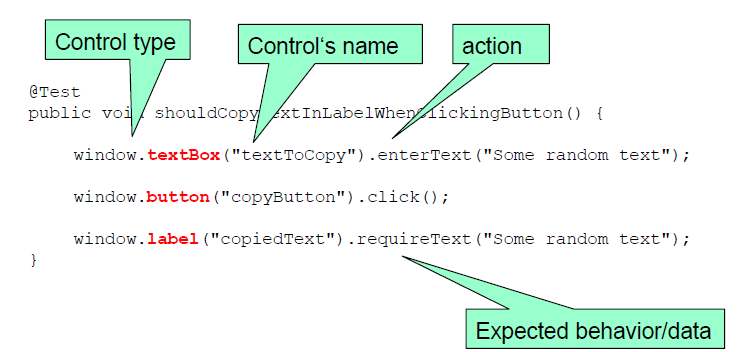
\includegraphics[scale=0.6]{FEST_Test.png}
\end{enumerate}
\begin{lstlisting}[language=Java,caption=FEST Beispiel 1.a, style=MyJavaStyle]
public class Hello extends JFrame {

    JLabel nameLabel = new JLabel("Please enter your name: ");
    JTextField nameTextField = new JTextField();
    JButton button = new JButton("Say Hello");
    JLabel welcomeLabel = new JLabel();

    public static void main(String[] args) {
        Hello hello = new Hello();
        hello.setVisible(true);
    }

    public Hello() {
        setLayout(new BorderLayout());
        JPanel namePanel = new JPanel();
        namePanel.setLayout(new FlowLayout());
        nameLabel.setAlignmentY(1.0f);
        nameTextField.setPreferredSize(new Dimension(300, 24));
        button.setPreferredSize(new Dimension(100, 40));
        welcomeLabel.setPreferredSize(new Dimension(350, 30));      
        welcomeLabel.setName("welcomeLabel");
        button.setName("helloButton");
        nameTextField.setName("nameTextField");

        button.addActionListener(new ActionListener() {

            @Override
            public void actionPerformed(ActionEvent arg0) {
                String name = nameTextField.getText();
                if (name == null || name.trim().isEmpty()) {
                    JOptionPane.showInternalMessageDialog(nameTextField,
                            "Please enter a name!");
                } else {
                    welcomeLabel.setText("Welcome " + nameTextField.getText());
                }}});
        namePanel.add(nameLabel);
        namePanel.add(nameTextField);
        add(BorderLayout.NORTH, namePanel);
        add(BorderLayout.WEST, button);
        add(BorderLayout.SOUTH, welcomeLabel);
        pack();
    }
}
\end{lstlisting}

\begin{lstlisting}[language=Java,caption=FEST Beispiel 1.b, style=MyJavaStyle]
package gui;

import org.fest.swing.*
import org.junit.*;

public class HelloTest {

    private FrameFixture window;

    @Before
    public void setUp() throws Exception {
        Hello frame = GuiActionRunner.execute(new GuiQuery<Hello>() {
            protected Hello executeInEDT() {
                return new Hello();
            }
        });
        window = new FrameFixture(frame);
        window.show();
    }

    @After
    public void tearDown() throws Exception {
        if (window != null) {
            window.cleanUp();
        }
    }

    @Test
    public void shouldCopyTxtInLabelWhenClickingButton() {
        window.textBox("nameTextField").enterText("Hans");
        window.button("helloButton").click();
        window.label("welcomeLabel").requireText("Welcome Hans");
    }
    
    @Test
    public void shouldGiveErrorWhenClickingButtonNoName() {
        window.textBox("nameTextField").enterText("");
        window.button("helloButton").click();
        window.optionPane().requireMessage("Please enter a name!");
    }
}
\end{lstlisting}
\pagebreak
\section{Web und Akzeptanztests}
\textbf{\Bold Anforderungen sind das Problem Nummer 1 beim Web und Akzeptanztesting}\\
\subsection{Herausforderungen bei Webtests}
\begin{itemize}
\item Teile der Applikation laufen im Browser ab
\item Wenig(er) Kontrolle über die Laufzeitumgebung
\item Browser-Inkompatibilit\"aten (IE vs. Firefox vs. Chrome vs. …)
\item Tools müssen auf verschiedene Browser zugreifen k\"onnen
\item Eigentlich wird ein verteiltes System getestet, da vom Browser immer auch http(s)-Requests auf den Server stattfinden.
\end{itemize}

\subsection{Selenium Testing System}
\subsubsection{Wie ist Selenium aufgebaut?}
Selenium besteht aus mehreren Teilen, nicht jedes Testprojekt ben\"otigt alle Teile:
\begin{itemize}
\item \textbf{\Bold Selenium IDE:} ein Capture/Replay-Plugin für Firefox erlaubt auch das Editieren der aufgenommenen Skripts
\item \textbf{\Bold Selenium WebDriver:} API um Browser programmatisch anzusteuern (z.B. aus Java, C-Sharp, PHP, Ruby…). Kann auch aufgenommene Skripts gegen andere Browser (�  Firefox) ausführen
\item \textbf{\Bold Selenium Server:} Koordiniert mehrere WebDriver um echte Lastszenarien zu simulieren.

\end{itemize}

\subsubsection{Was bietet Selenium?}
\begin{itemize}
\item Selenium bietet Capture/Replay Funktionalit\"at
\item Generiert Skript, das editierbar ist
\item Da HTML verwendet wird, k\"onnen Events einzelnen Elementen zugeordnet werden
\item Keine Aufzeichnung von GUI-Koordinaten n\"otig\\
(ABER: Jedes Element muss eindeutige ID haben!)
\end{itemize}

\subsection{Die Kundensicht}
Für den Kunden stehen die Gesch\"aftsprozesse immer im Vordergrund.\\\\
\textbf{\Bold Definition:} Ein Gesch\"aftsprozess ist eine Folge von koordinierten Aufgaben und Aktivit\"aten, die das Ziel haben ein Gesch\"aftsresultat zu realisieren.

\subsubsection{Eigenschaften eines Gesch\"aftsprozesses}
\begin{itemize}
\item Nach Aussen gerichtet (beschreibt beobachtbares Verhalten)
\item Benutzeranforderung
\item Wiederholte Durchführung
\item Unabh\"angig von GUI
\end{itemize}

\subsubsection{Feedback}
Ein frühes Feedback gegenüber dem Kunden, hilft eine Software korrekt und wunschgem\"ass zu entwickeln.\\\\
\textbf{\Bold Problem:} Unittests sind nicht wirklich aussagekr\"aftig und GUI-Test werden erst sp\"at im Projekt gemacht. Daher sollten früh im Projekt mit dem Kunden zusammen Akzeptanztest erstellt und definiert werden.

\subsubsection{Herausforderung beim Erstellen von Akzeptanztests}
\begin{description}
\item[\Bold {Prozesse}] \hfill \\ 
	Wie k\"onnen Prozesse als Test beschrieben werden?
\item[\Bold {Die Sprache}] \hfill \\
	Entwicklersprache vs. Benutzersprache
\item[\Bold{Komplexit\"at}] \hfill \\
	Formalisierung der Anforderungen
\item[\Bold{Abh\"angigkeiten}] \hfill \\
	Prozessintern\\
	$\rightarrow$ Teilaktivit\"aten h\"angen von einander ab\\
	Prozessextern\\
	$\rightarrow$ High-Level Prozesse bauen auf Low-Level Komponenten und externen Systemen auf
\item \Bold {Infrastruktur ist nicht verf\"ugbar}
\item[\Bold {Automatisierung}] \hfill \\ 
	Essentiell f\"ur Regressionstests
\end{description}

\subsection{FIT - Framework for Integrated Testing}
\subsubsection{Einleitung}
\Bold {Ziel:}
\begin{itemize}
\item Vermeidung von Anforderungsfehlern durch Einrichtung einer fr\"uhen Feedback-Loop zwischen Entwicklern und Benutzern auf Testbasis
\end{itemize}
\Bold {Konzepte:}
\begin{itemize}
\item Ausf\"uhrbare Use Cases und Workflows�
\item F\"ur Kunden/Benutzer verst\"andlich und durch diesen erstellbar
\item Konkrete Beispiele (Testing by Example�)
\end{itemize}

\subsubsection{Architekturkonzept}
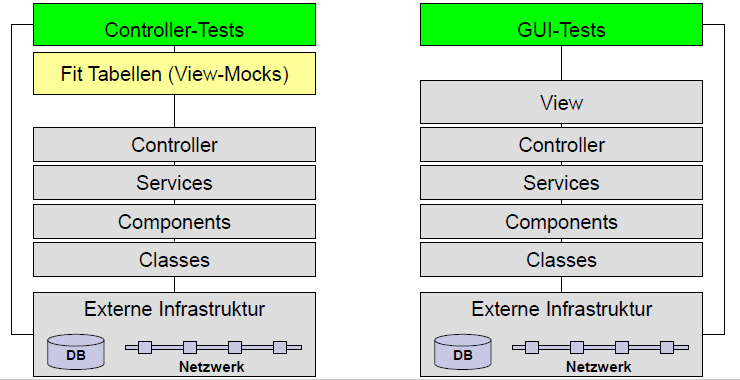
\includegraphics[scale=0.5]{FIT_Architekturkonzept.png}

\subsubsection{Vorgehenskonzept}
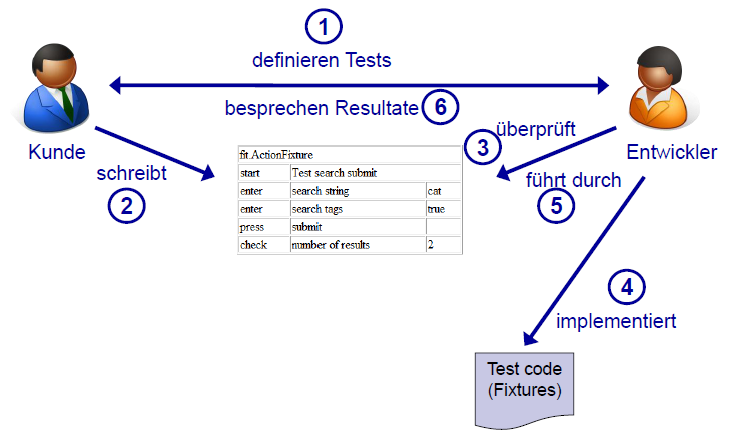
\includegraphics[scale=0.5]{FIT_Vorgehenskonzept.png}

\subsubsection{Hinweise zur Testspezifikation}
\begin{itemize}
\item Auswahl der richtigen Tabellen-Typen
\item Sprache des Benutzers w\"ahlen
\item Lesbare Testnamen\\
Statt Fixtures.TestSearchSubmit$ \rightarrow$ �Test Search Submit
Fit generiert den Klassennamen (CamelCase, Graceful Names)
\item Initialisierung/Setup und Aufr\"aumen der Testumgebung/TearDown wird unterst\"utzt.
\item Kunde und Entwickler erarbeiten Tests gemeinsam
\end{itemize}

\subsubsection{FIT Fixtures}
Die Testf\"alle werden bei Fit in HTML-Tabellen definiert. Die Anbindung an das zu testende Programm erfolgt über Java-Klassen, die "Fixtures" genannt werden, und die bestimmte Fit-Fixture-Klassen erweitern.\\
Es gibt die drei Basis-Fixtures ColumnFixture, RowFixture und ActionFixture. Wenn auf Zusatzbibliotheken (z.B. FitLibrary) zurückgegriffen wird, stehen zus\"atzlich noch viele weitere Fixtures zur Verfügung (z.B. DoFixture).\\
Die folgende Tabelle beschreibt die drei Basis-Fixture-Typen:\\
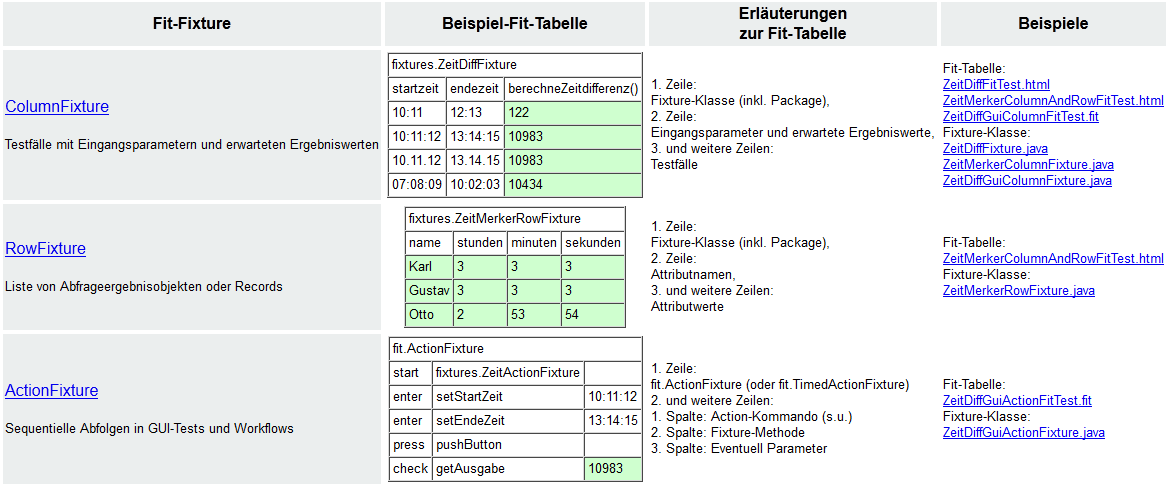
\includegraphics[scale=0.55]{FIT_Fixtures.png}

\subsubsection{Testimplementierung}
Von den Tabellen zu der Implementierung:\\
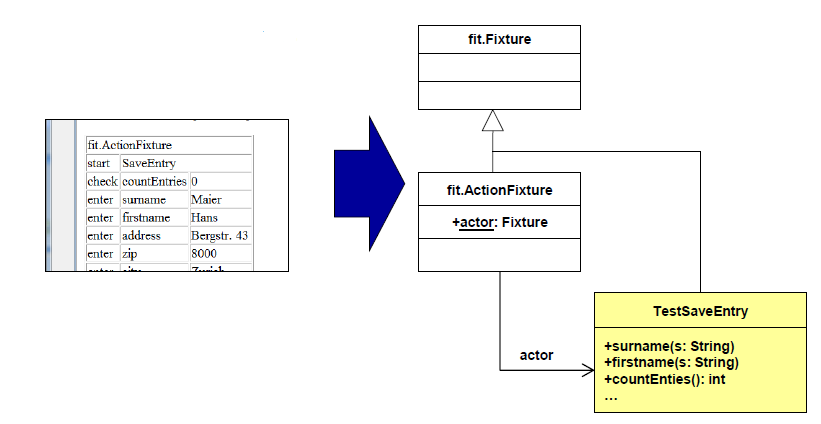
\includegraphics[scale=0.6]{FIT_TestImplementierung.png}

\subsubsection{Hinweise zur Testimplementation}
\begin{itemize}
\item Auch Testcode muss gewartet werden
\item Prozesskontext definieren
	\begin{itemize}
		\item Daten\"ubergabe \"uber statics 
	\end{itemize}
\item Fit Fixtures f\"ur dom\"anenspezifische Bed\"urfnisse verf\"ugbar (z.B. Web, DB…)
\item Falls notwendig erweiterbar
	\begin{itemize}
		\item Neue Befehle durch Ableitung von ActionFixture
		\item Eigene Fixture-Klassen
	\end{itemize}
\item Auf Trennung zwischen Businesslogik und Testcode achten
	\begin{itemize}
		\item Fit-Tests in separatem Test-Verzeichnis
	\end{itemize}
\end{itemize}

\newpage
\section{Zus\"{a}tzlicher Sourcecode}
\begin{lstlisting}[language=Java,caption=JUnit-Test mit Javadoc, style=MyJavaStyle]
  /**
   * Test method for {@link ch.fhnw.edu.rental.model.Movie#Movie(java.lang.String, 
   * ch.fhnw.edu.rental.model.PriceCategory)}.
   * @throws InterruptedException must not be thrown
   */
  @Test
  public void testMovieStringPriceCategory() throws InterruptedException {
    // get time before object creation
    Date before = new Date(Calendar.getInstance().getTimeInMillis());
    // spend some time to be able to detect differences in timestamps
    Thread.sleep(10);

    // now allocate new instance
    Movie m = new Movie("A", RegularPriceCategory.getInstance(), 18);
    // get time after object creation
    Thread.sleep(10);
    Date after = new Date(Calendar.getInstance().getTimeInMillis());
    
    assertNotNull(m);
    assertEquals("A", m.getTitle());
    assertEquals(RegularPriceCategory.class, m.getPriceCategory().getClass());
    Date releaseDate = m.getReleaseDate();
    assertNotNull(releaseDate);
    assertTrue(before.before(releaseDate));
    assertTrue("Expected release date to be earlier.", after.after(releaseDate));
    assertFalse(m.isRented());
    assertEquals(18, m.getAgeRating());
  }
\end{lstlisting}
\begin{lstlisting}[language=Java,caption=Junit-Test mit Mock-Testing, style=MyJavaStyle]
    @Test
    public void testRemoveLowStockListener() {
        expect(m.getTitle()).andStubReturn("Tarzan");
        expect(l.getThreshold()).andReturn(2).once();
        l.stockLow(m, 2);
        
        replay(m);
        replay(l);
        
        st.addLowStockListener(l);
        
        st.addToStock(m);
        st.addToStock(m);
        st.addToStock(m);
        st.removeFromStock(m);
        
        st.removeLowStockListener(l);
        st.addToStock(m);
        st.removeFromStock(m);
        
        verify(l);
        verify(m);
    }
\end{lstlisting}

\begin{lstlisting}[language=Java,caption=Junit-Test mit korrekter Verwendung von fail(), style=MyJavaStyle]
    @Test
    public void testExceptionRental() throws InterruptedException {
        Rental r = null;
        try {
            r = new Rental(null, m1, 1);
            fail();
        } catch (NullPointerException e) {
            assertEquals(NULLMESSAGE, e.getMessage());
        }
\end{lstlisting}

\begin{lstlisting}[language=Java,caption=Methode mit JavaDoc, style=MyJavaStyle]
  /**
   * removes a movie from the stock.
   * @param movie the movie to remove from the stock.
   * @return the number of items of this movie in stock after this operation.
   */
  public int removeFromStock(IMovie movie) {
    Integer i = stock.get(movie.getTitle());
    int inStock = (i == null) ? 0 : i;
    if (inStock <= 0) { throw new MovieRentalException("no video in stock"); }
    stock.put(movie.getTitle(), --inStock);
    notifyListeners(movie, inStock);
    return inStock;
  }
\end{lstlisting}

\begin{lstlisting}[language=Java,caption=Log4j, style=MyJavaStyle]
    public void setReleaseDate(Date aReleaseDate) {
        logger.trace("entering Movie.setReleaseDate");
        if (this.releaseDate != null) {
            IllegalStateException e = new IllegalStateException();
            logger.error("Exception:", e);
            throw e;
        }
        this.releaseDate = aReleaseDate;
        logger.debug("releaseDate: " +  this.releaseDate);
        logger.trace("exiting Movie.setReleaseDate");
    }
\end{lstlisting}

\end{document}